\chapter{INTRODUCTION}
\label{chp:1}

\section{Global Renewable Energy Status}
Renewable energy is still one of the hottest topics in the power area. The share of the renewable energy systems has been reached significant levels. At the end of 2016, the renewable power capacity has reached 2011 GW throughout the world including hydropower plants.\cite{InternationalRenewableEnergyAgency2017}  The renewable capacity for the leading countries is given in the Figure \ref{renewablecap}.Almost half of this capacity belongs to four leading countries namely; China, USA, Brazil and Germany. \par
\begin{figure}[h!]
	\centering
	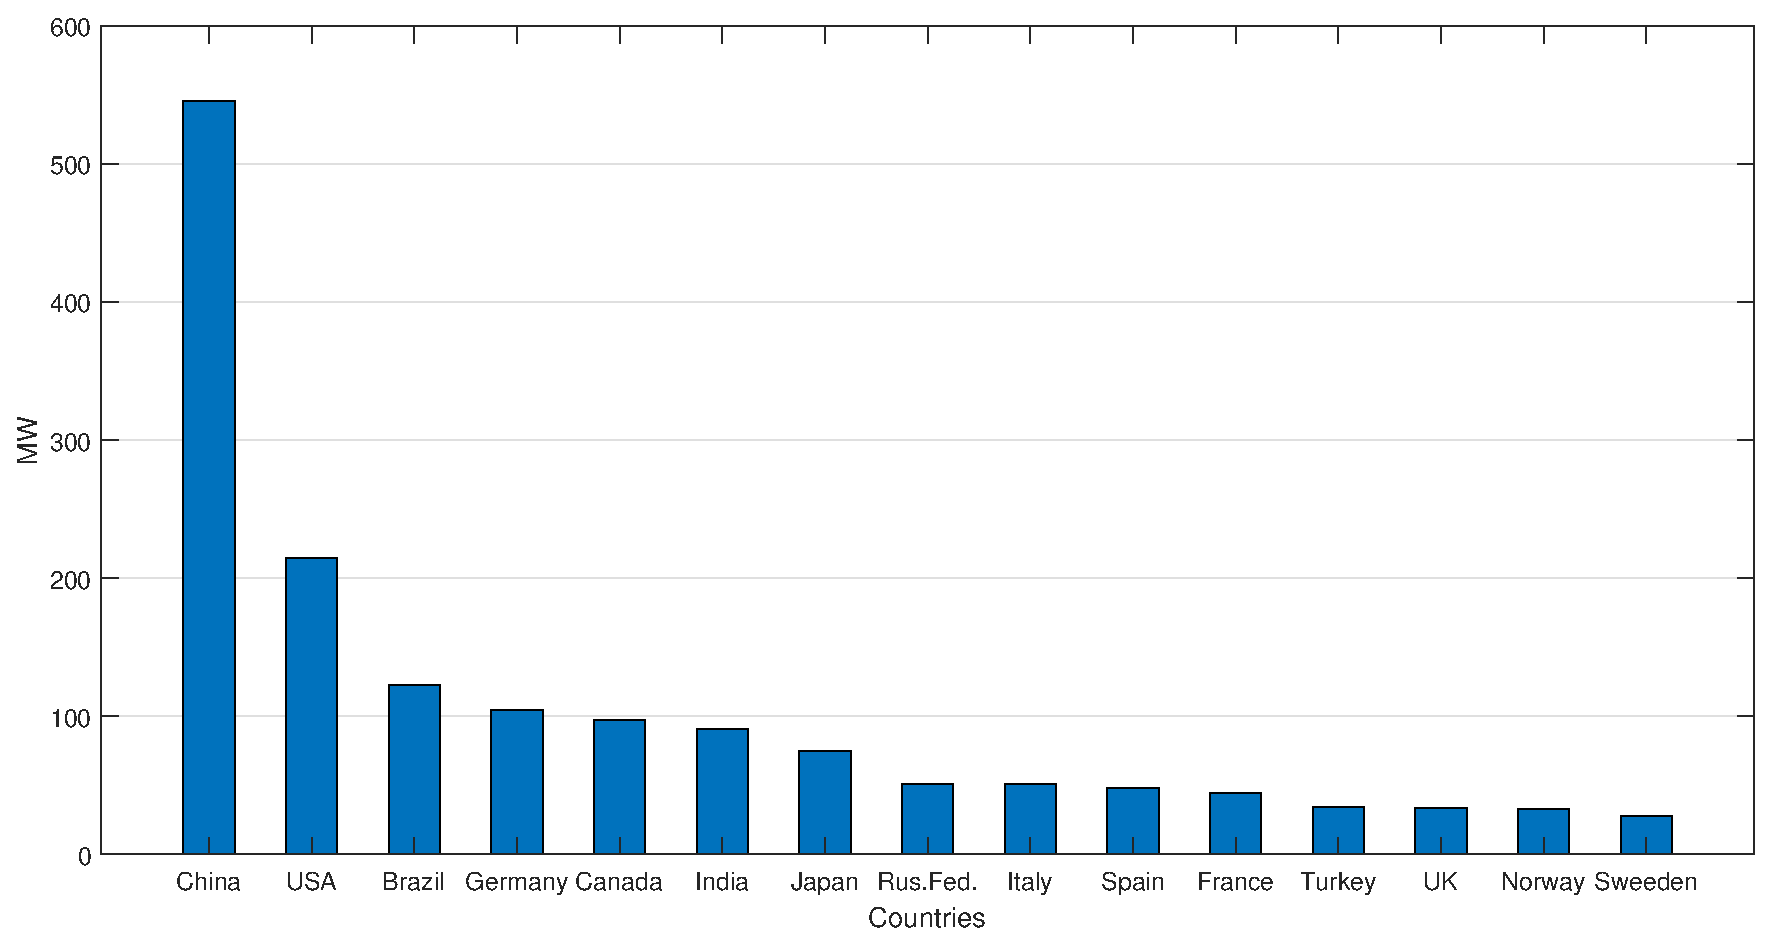
\includegraphics[scale=0.47]{renewablecapacity.eps}
	\caption{Installed Renewable Energy Capacity of Leading Countries in 2016\cite{InternationalRenewableEnergyAgency2017}}
	\label{renewablecap}
\end{figure}
\begin{figure}[h!]
	\centering
	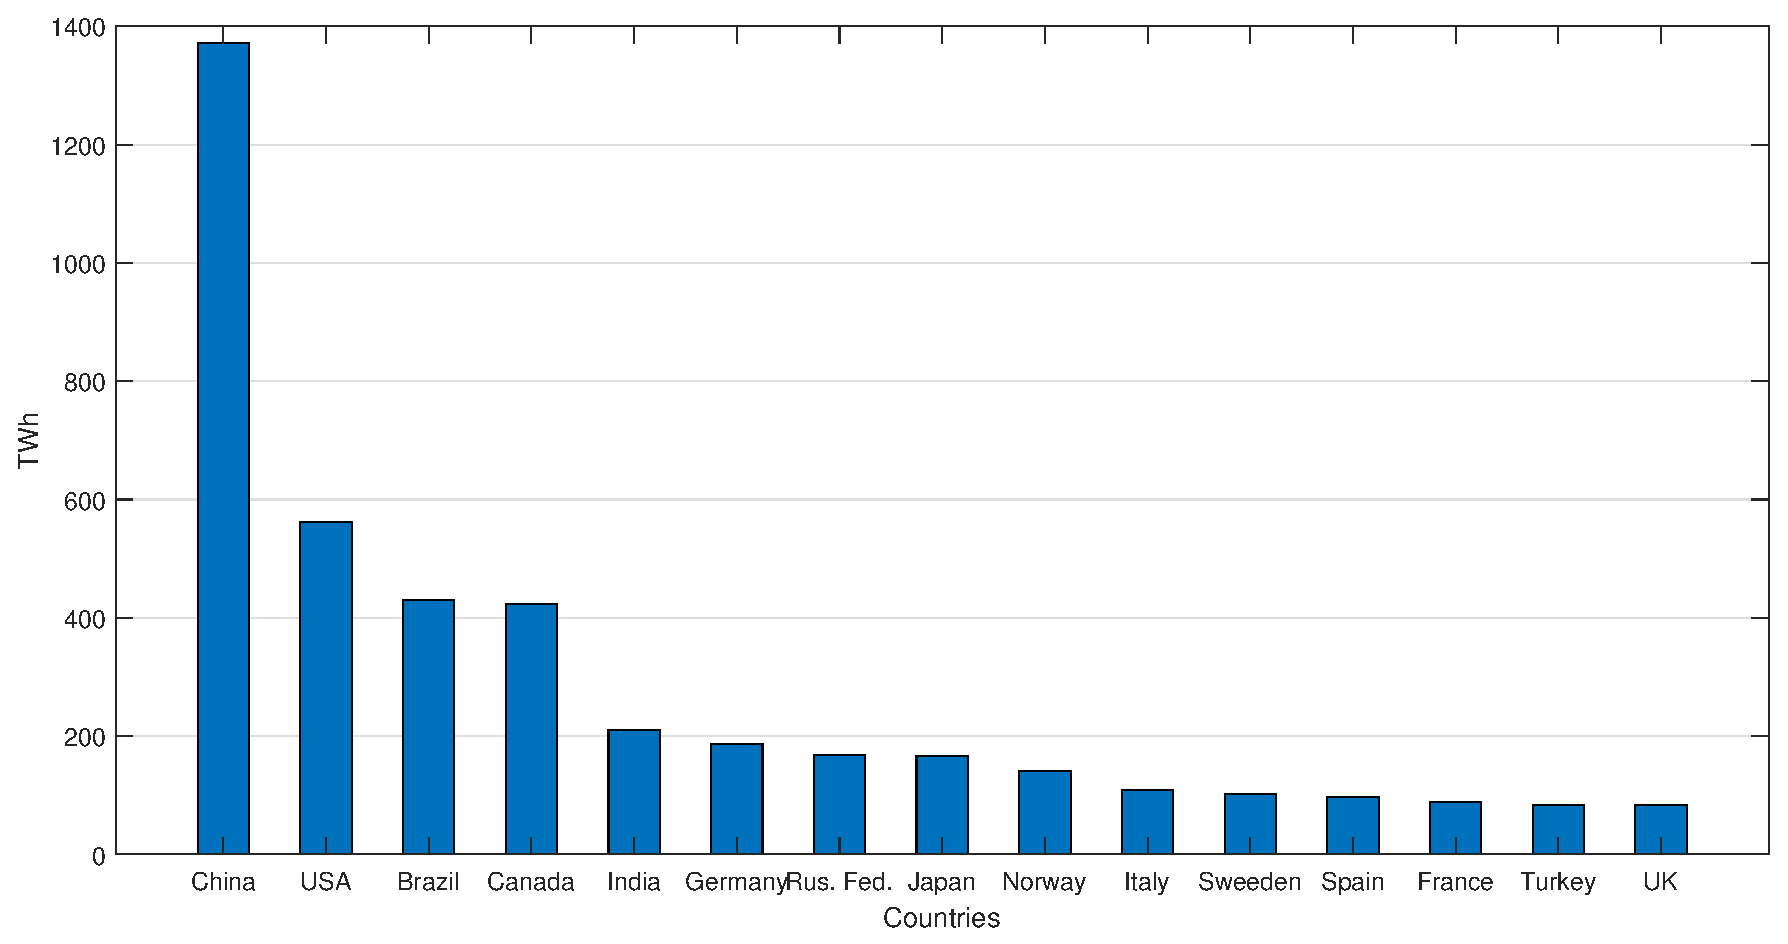
\includegraphics[scale=0.47]{renewableproduction.eps}
	\caption{Renewable Energy Production of Leading Countries in 2016 \cite{InternationalRenewableEnergyAgency2017}}
	\label{renewablepro}
\end{figure}
Figure \ref{renewablepro} shows the energy production from renewable energy systems. It is clear that China, USA and Brazil produces highest amount of energy from renewable since they already have the highest installed capacity. However, India and Canada produces more energy than Germany even though Germany has more installed capacity. This result is due to the fact that renewable energy system production is dependent on parameters such as solar radiation and wind speed depending on the renewable source.
\subsection{EU 2020 Goals}
In 2008, 20 20 by 2020-Europe's Climate Change Opportunity report has been released by EU Commission and two key targets are set for 2020 \cite{EuropeanCommission2008}: 
\begin{itemize}  
	\item At least 20 \% reduction in greenhouse gases (GHG) by 2020
	\item Achieving 20\% renewable energy share in energy consumption of EU by 2020
\end{itemize}
The Renewable Energy Directive is published in 23 April 2009. This directive has set national binding targets for EU countries in order to accomplish the 20\% renewable energy target for EU and 10 \% target for the renewable energy usage in the transport. \cite{EuropeanParliament2009} As a result, each EU country has been determined their national action plans. In order to achieve the 20 \% target, each member state determine their own targets ranging from 10\% in Malta to 49\% in Sweeden. 
According to the latest release by Eurostat, renewable share of the EU in energy consumption has reached 17 \% in 2016 \cite{States2016}. Moreover, eleven of EU member states has already achieved their 2020 targets. Renewable shares of EU members are shown in Figure \ref{EUtargets}.
\begin{figure}[h!]
	\centering
	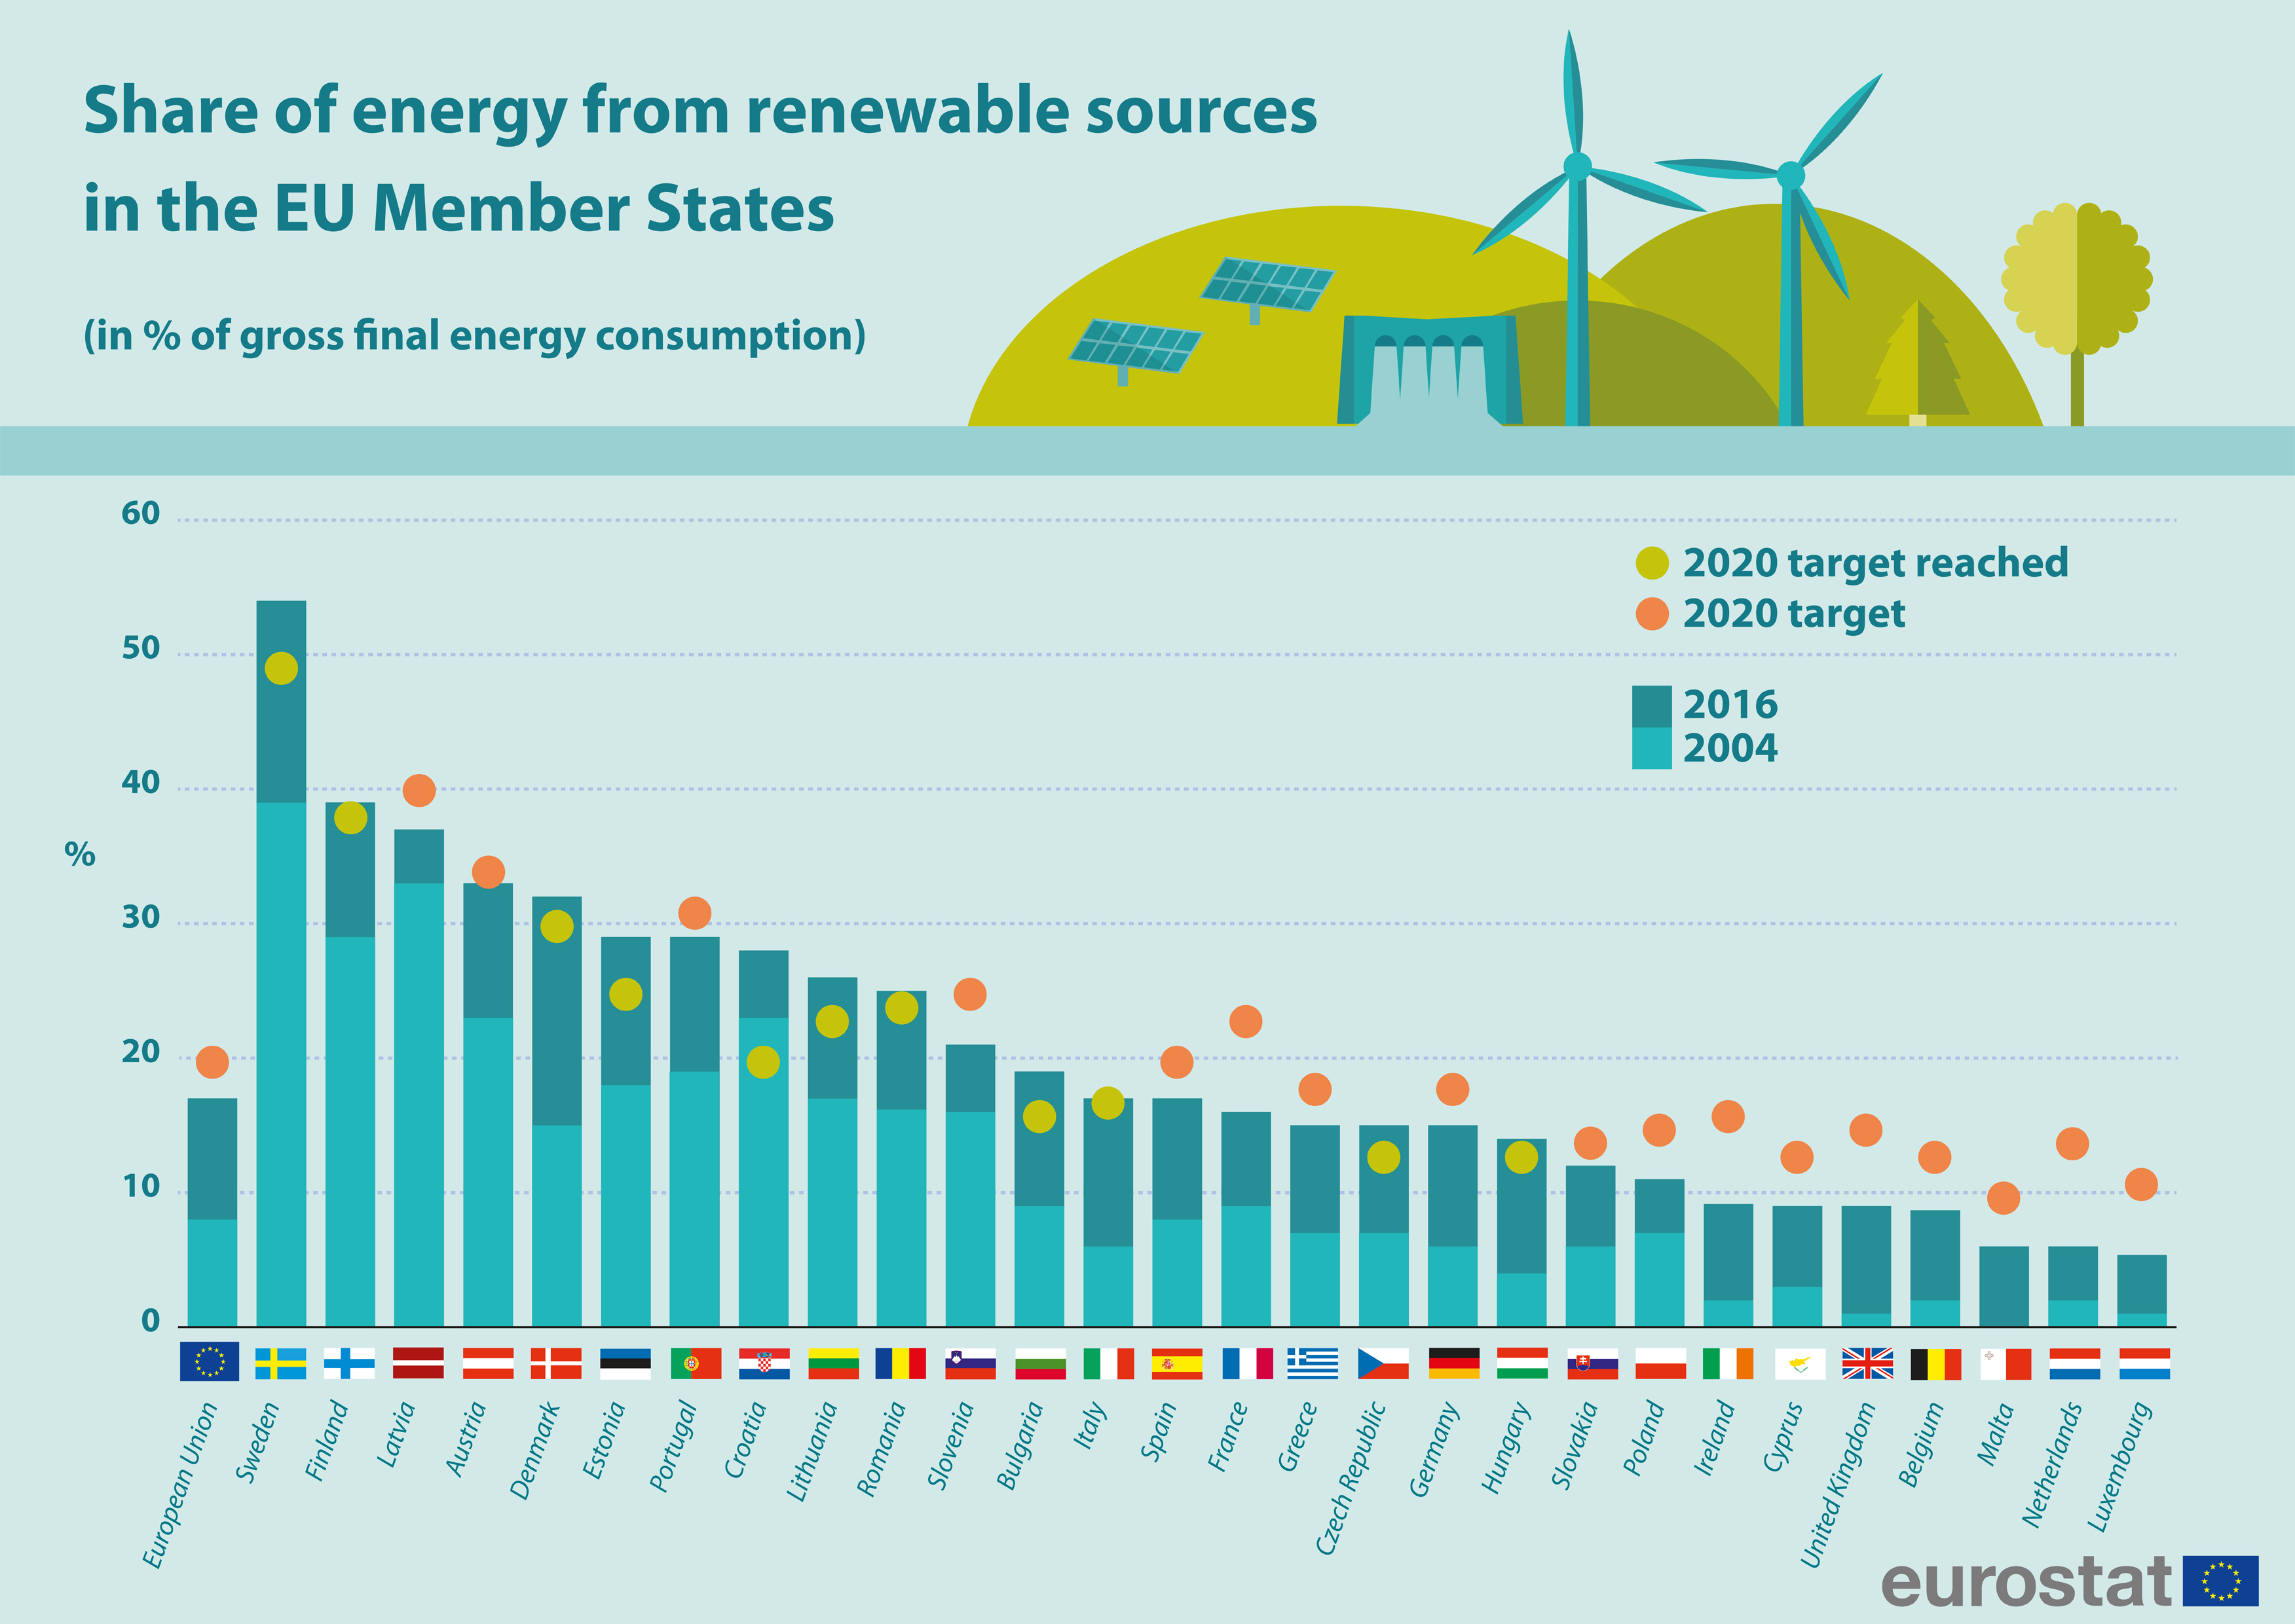
\includegraphics[scale=0.12]{Figure_1-Share_of_energy_from_renewable_sources_2004-2016.png}
	\caption{Renewable Targets of EU Member States\cite{States2016}}
	\label{EUtargets}
\end{figure}


\subsection{Wind Energy Status}
Wind power has the highest share in the renewable energy except for hydropower. The wind power capacity at the end of 2016 has reached 467 GW worldwide. The wind power capacity of the leading countries are given in the Figure \ref{windcap}. China and USA have also the highest installed capacities in the wind power. Moreover, it should also be noted that the share of the wind power in the total installed capacity is more important that total wind power capacity
\begin{figure}[h!]
	\centering
	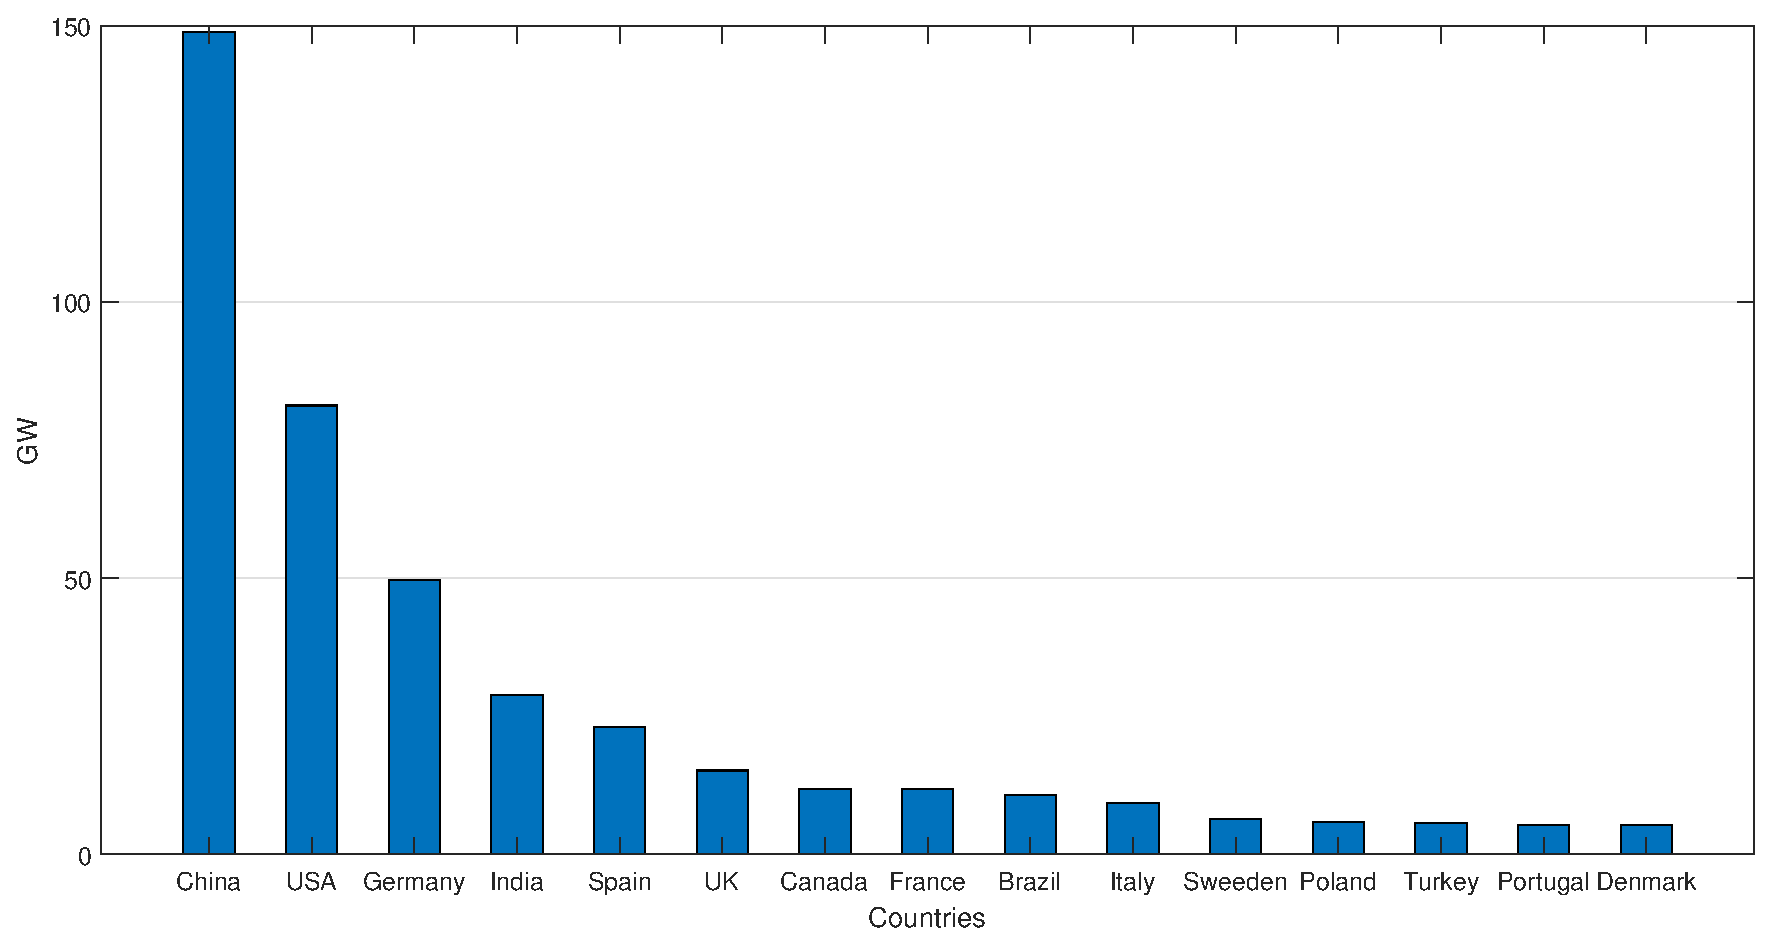
\includegraphics[scale=0.47]{windcapacity.eps}
	\caption{Wind Power Capacity of Leading Countries in 2016\cite{InternationalRenewableEnergyAgency2017}}
	\label{windcap}
\end{figure}
The energy production from wind energy is shown in the Figure \ref{windpro}. Even though China has the highest wind power capacity,  USA generates more energy from wind than any other country. 
\begin{figure}[h!]
	\centering
	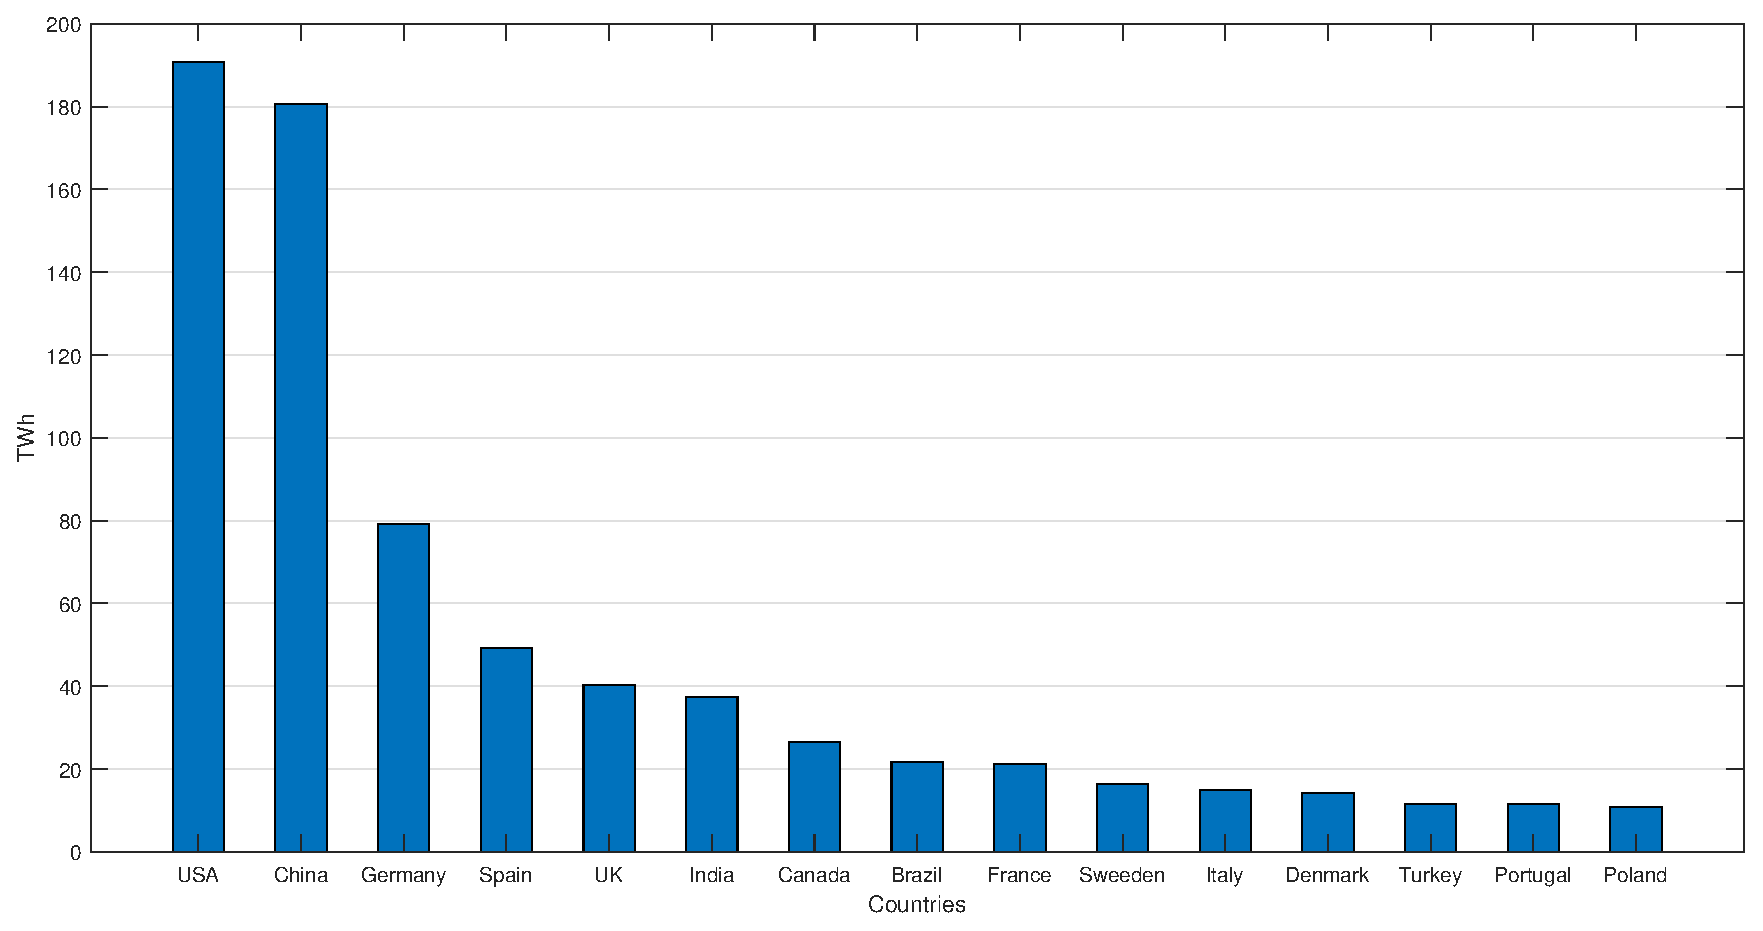
\includegraphics[scale=0.47]{windproduction.eps}
	\caption{Wind Power Production of Leading Countries in 2016\cite{InternationalRenewableEnergyAgency2017}}
	\label{windpro}
\end{figure}


\section{Global Renewable Energy Future}
The share of renewable energy is increasing each passing day. Today, reports arguing the possibility of even 100\% renewable energy region by region is published\cite{REN212017d}. The renewable energy reports estimate the share of renewable energy in the total energy consumption for 2030 and 2050. Figure \ref{EU2030} shows the EU renewable energy share for 2030. Moreover, the report published by IRENA (International Renewable Energy Agency) estimates the share of renewable energy in EU as 24\% by 2030 which is below proposed target of 27\%\cite{IRENA2014}.
\begin{figure}[h!]
	\centering
	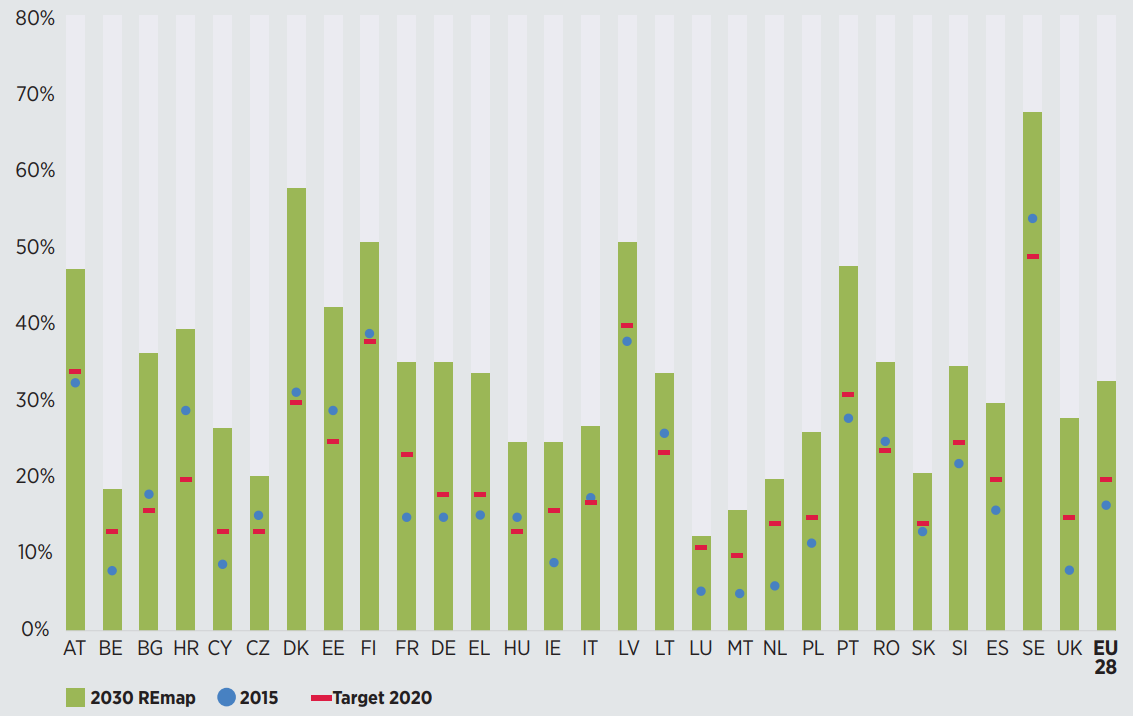
\includegraphics[scale=0.47]{EU2030.png}
	\caption{Renewable energy share in total energy consumption by EU for 2015, 2020 targets and 2030 potential according to REmap \cite{EuropeanCommission2018}}
	\label{EU2030}
\end{figure}
\begin{figure}[h!]
	\centering
	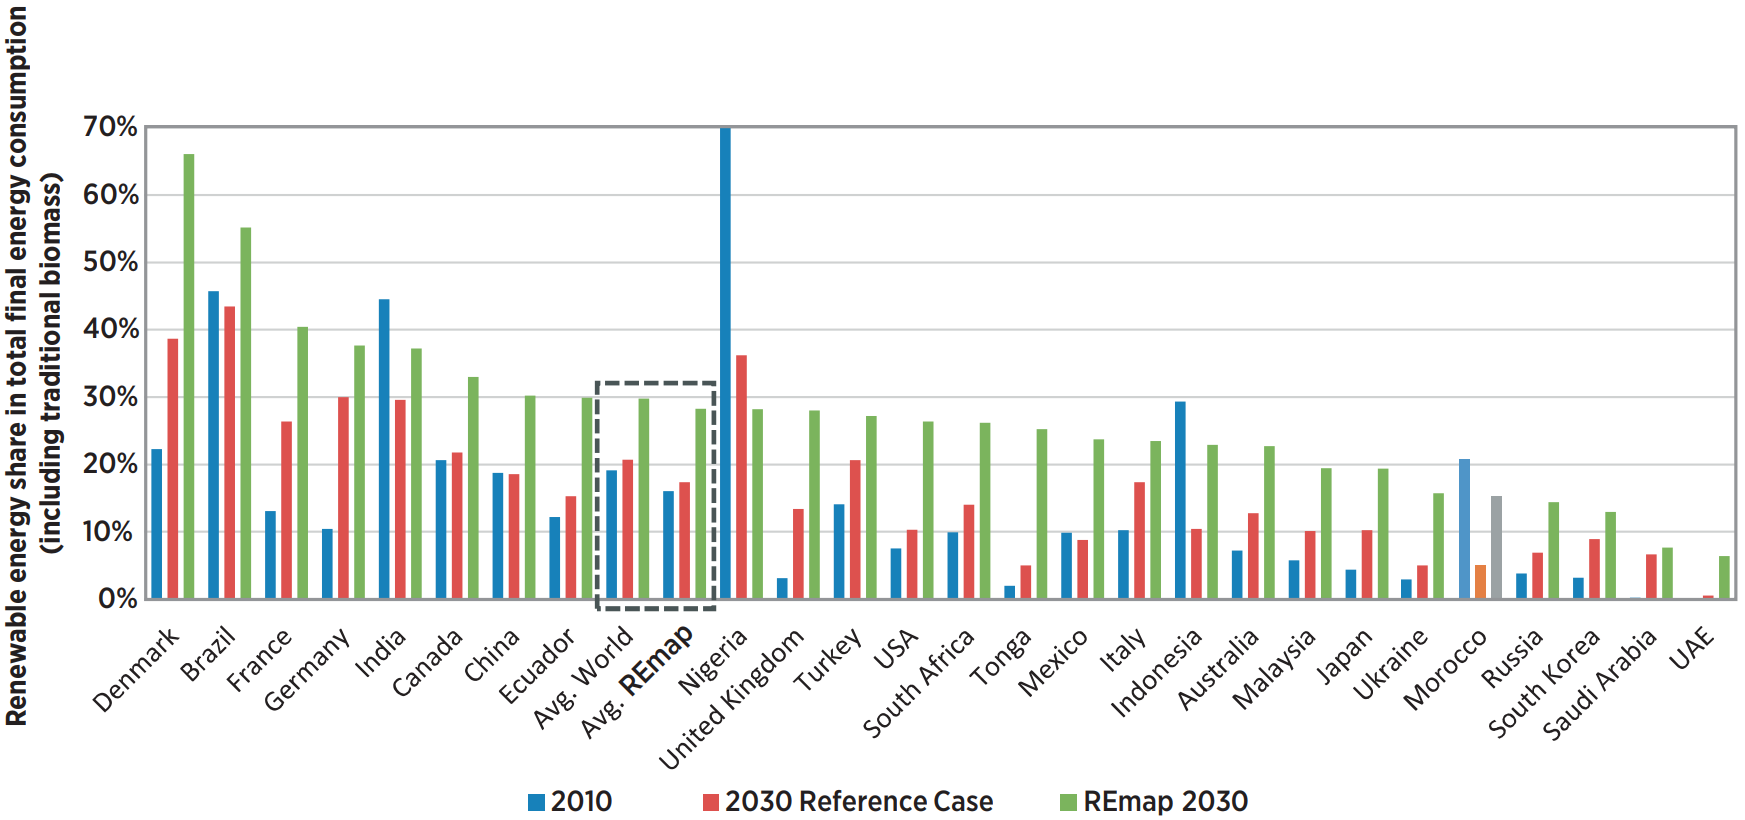
\includegraphics[scale=0.3]{2030map2.png}
	\caption{Renewable energy shares for 2010, 2030 Reference Case and 2030REmap \cite{IRENA2014}}
	\label{2030map}
\end{figure}
Renewable shares of REmap countries in 2010, 2030 reference case and 2030REmap and the world average is also shown in Figure \ref{2030map}. The only country whose renewable energy decreases in the 2030 is Nigeria. The reason is the main source of energy in Nigeria is biogas for the time being. However, the renewable share is expected to decrease dramatically as the industry switches to natural gas.
\section{Renewable Energy Problems}
It is an undeniable fact that renewable energy systems are advantageous in terms of global warming and carbon dioxide emission. Nonetheless, they also have disadvantages to the system operators due to intermittent energy generation. With the large penetration of intermittent sources, electric grid will face with transmission system issues as overloaded transmission lines, changes on the protection and control in the distribution system, greater level of power-factor control and low voltage ride-through (LVRT) requirements \cite{Ipakchi2009}.\\
Another challenge of renewable energy systems  is the power system frequency stability. Since the frequency of the power system depends on the balance between generation and consumption, grid operators are responsible for adjusting the generation in order to maintain a constant frequency. However, the renewable energy generation is strictly dependent on the renewable source i.e. solar radiation or wind speed. Therefore, renewable systems makes the system operation harder due to their intermittent and uncertain power generation profiles. Moreover, as the renewable systems with power electronics interface increase in the electricity grid, the grid equivalent inertia decreases. In \cite{Gautam2011}, the reduced grid inertia due to the high DFIG wind turbine penetration is emphasized. Moreover, the results of the reduced grid inertia following a disturbance is listed as: 
\begin{itemize}
	\item increased effective aggregated angular acceleration of synchronous machines which require high restoring forces
	\item high rate of change of frequency and hence, decreased frequency nadir
\end{itemize}
It should be noted that this problem is not specific to DFIG wind turbines but renewable energy systems which are connected to grid with power electronics. Conventional synchronous generators rotates with synchronous speed which is proportional to grid frequency. If the grid frequency decreases, then the synchronous speed also decreases. In this case, the generator active power is increased inherently due to kinetic energy extraction from the generator inertia. The increase in active power provides action time for primary controllers and crucial for frequency stability. Type-1 and Type-2 wind turbines are directly connected to grid. Hence, the frequency deviations affects the active power output of such wind turbines\cite{Muljadi2012}. Nonetheless, active power output of renewable energy systems with power electronics such as Type-3 and 4 wind turbines and photovoltaic systems is not affected from the grid frequency deviations. Therefore, these system have no contribution to the grid inertia whether the system includes inertia or not. Hence, the aggravated grid inertia is reduced with the penetration of renewable energy sources. The comparison for different type of generators is given in \cite{VanDeVyver2016} and listed in Table \ref{generatorcomparison}. Another reason for the decrease in the grid inertia is the de-commitment or dispatch of the conventional sources due to economic concerns. Since the renewable energy has the lowest cost for energy production, it preferred instead of conventional generators. As a result, conventional generators are dispatched to a lower generation profile or taken-off from operation. 
\begin{table}[h!]
	\centering
	\begin{tabular}{lc}
				\hline
		\multicolumn{1}{c}{\textbf{Type of the generator}}                                                                            & \textbf{Inertial Response Behaviour} \\ \hline
		Conventional Synchronous Generator                                                                                            & ++                                   \\
		Fixed Speed Induction Generator (FSIG)                                                                                        & +                                    \\
		Doubly Fed Induction Generator (DFIG)                                                                                         & -                                    \\
		\begin{tabular}[c]{@{}l@{}}Variable Speed Wind Turbine Generator\\ (Connected with Full Scale Power Electronics)\end{tabular} & None                                 \\ \hline
	\end{tabular}
	\caption{Comparison of Different Type of Generators for Inertial Response Behaviour}
	\label{generatorcomparison}
\end{table}
\section{Literature Review}
Studies regarding inertial support date back to early 2000s. In the study \cite{Lalor2004}, the effect of the increasing wind energy penetration has been investigated. The study concludes that increasing share of wind energy increases the primary reserve requirement for the successful grid operation. The increased frequency deviations, especially in light load conditions (high wind generation with low consumption scenario) can be mitigated in the system as long as the wind generation provides inertia support. Study in \cite{Ekanayake2003} states that DFIG wind turbines are de-coupled from power system resulting in no contribution to system inertia. A supplementary loop is proposed for reinstating the machine inertia. Moreover, in \cite{Ekanayake2004}, performance of the  supplementary control loop is evaluated with the comparison of the inertial support of a fixed-speed wind turbine. The proposed control loop has been validated in \cite{Morren2006} and compared with the droop control in \cite{Morren2006a}. \par 
It is an undeniable fact that renewable energy systems are the most economical way of producing electrical energy due to absence of any fuel cost. Therefore, they are to be operated in their rated power. However, they have to curtail their power in order to leave a margin for droop control. Droop control by wind energy is also studied in the literature. In \cite{Muljadi2012}, the inertial support of different type of wind turbines is compared. It is concluded that the Type-4 wind turbines are able to perform better performance for inertial support due to the power electronics interface. Moreover, combination of inertial support and droop control produces better results in these wind turbines. 
\section{Thesis Motivation}
The frequency of the electric grid depends on the balance between generation and consumption. Grid operators are responsible for maintaining this balance so that frequency of the grid is maintained between allowed dead-band. In order to achieve this purpose, power generation is adjusted according to the consumption value. However, the balance between supply and demand might be disturbed with unintentional generator trip or instant load connections. Grid frequency decreases such instants until the generation is increased to arrest the frequency. Inertia of the electric grid provides additional power from the stored kinetic energy and avoid the system frequency from decreasing down very fast. That is called as inertial support and it is very important for power system frequency stability.\\
Although renewable energy systems are beneficial for environmental concerns and lower energy cost, higher renewable penetration also brings operational challenges for system operators. One of the most important problem that comes with renewable energy is the power system frequency stability. With the high renewable penetration, grid aggravated inertia decreases. As a result, grid frequency deviates steeper for disturbances. To avoid steeper frequency declines in the grid, all generation technologies should provide inertial support for the frequency disturbances.\\
Wind energy systems, especially variable speed wind turbines with full scale power electronics are the most promising renewable energy systems that can contribute to grid frequency stability thanks to their high inertia in their blades and generator and also their back-to-back converters that give ability to control its active power. Therefore, wind energy conversion systems are required to participate in ancillary services for frequency stability in order to reach a stable power system network in the upcoming future.


















